\documentclass[12pt]{article}
\usepackage[utf8]{inputenc}
\usepackage{graphicx} % Allows you to insert figures
\usepackage{amsmath} % Allows you to do equations
\usepackage{fancyhdr} % Formats the header
\usepackage{geometry} % Formats the paper size, orientation, and margins
\usepackage{caption}
\usepackage{subcaption}
\usepackage[style=authoryear-ibid,backend=biber]{biblatex} % Allows you to do citations - does Harvard style and compatible with Zotero
\addbibresource{Example.bib} % Tells LaTeX where the citations are coming from. This is imported from Zotero
\usepackage[english]{babel}
\usepackage{csquotes}
\renewcommand*{\nameyeardelim}{\addcomma\space} % Adds comma in in-text citations
\linespread{1.25} % About 1.5 spacing in Word
\setlength{\parindent}{0pt} % No paragraph indents
\setlength{\parskip}{1em} % Paragraphs separated by one line
\renewcommand{\headrulewidth}{0pt} % Removes line in header
\geometry{a4paper, portrait, margin=0.7in}
\setlength{\headheight}{14.49998pt}
\usepackage{titlesec}
\titlespacing{\subsection}{1pt}{\parskip}{-\parskip}

\usepackage{enumitem}
\begin{document}
	\begin{titlepage}
		\begin{center}
			\vspace*{5cm}
			
			\Huge{Weekly Reports}
			
			\vspace{0.5cm}
			\LARGE{Mehmani Research Group}
			
			\vspace{3 cm}
			\Large{}
			
			\vspace{0.25cm}
			\large{Nicolás Bueno Zapata}
			
			\vspace{3 cm}
			\Large{Spring 2022}
			
			\vspace{0.25 cm}
			\Large{The Pennsylvania State University}
			
			
			\vfill
		\end{center}
	\end{titlepage}
	
	\setcounter{page}{2}
	\pagestyle{fancy}
	\fancyhf{}
	\rhead{\thepage}
	\lhead{Nicolas's Reports}
	
	\section*{Jan 30, 2022}
	 During this week I was focoused on testing my LBM code for a single component and multiphase conditions. For validation, I looked for other available codes from the postdoc, Cheng, and codes available in the Dr. Ayala's research group. I had to redefine some objects in my code to be able to pursue the next modeling objectives as:
		
	\begin{itemize}
		\item Have different relaxation parameters for every component
		\item Have more than one force applying to our components 
		\item The components also have the propety "pseudopotential"

	\end{itemize}

	I was reading how to model two immiscible components through LBM, and I discover that the treatment of Cheng is quite different (valid, though) from the proposed in Kruger's book. I created a new routine with a different Shan-Chen force implementation (each component uses its own pseudopotential) for immiscible displacement, because I want to be able to simulate a case where I inject a single component that displaces the other, although I just realize that I need to specify the composition of my injecting fluid for all the boundary conditions we have specified. In single component, specifing the pressure is equivalent to specify the density. However, for multi-component, we need to provide the amount of each component at that pressure to be able to have a solvable system.
	
	I decided to keep track of all the different options and equations inside the code, and I started to write my own LBM document to explain to myself and future users, what are the equations implemented and the logic behind them. 
	
	It has been difficult to balance the time for research, coding, and reading papers where to inspire for research ideas and applications. I am still trying to find the correct point in this semester, as all the courses are kind of related to my thesis, and all deserve the same degree of attention. 
	
	\pagebreak
	
	\section*{Feb 6, 2022}
	
	\subsection*{Things that were done}
	This week started the full implementation of the multi-relaxation-times collision operator for my LBM model. Despite the first coding stage, I had programmed classes for collisionMRT operator and the lbmParameter object, these two were somehow in conflict, as the Fortran polymorphism is somehow more strict than in C++, so I had to arrange the code to account for generalization in the main routines, who do not know in principle, which type of object are they calling to. I read about LAPACK, a library to handle linear systems in Fortran, that could be useful for other problems and applications using the code in development. 
	
	Another advance in this matter was the two-phase flash algorithm that is almost working in C++. The purpose of this code is to have my own library for thermodynamic analysis of mixtures (solve stability, n-phase flash, envelopes, bubble points) that can give insights in how to set a simulation case for the LBM code. The novelity with this code is that is connected with Matplotlib, library from Python, so it can be used any plot command from there in C++. I would like to improve the Subsequent Substitution Method by a Newtonian algorithm using the C++ Library, Eigen, to solve linear systems of equations. 
		
	\subsection*{Difficulties}
	This semester, as particularly intense, has been difficult to balance between study and working times. However, I have managed to take advantage of the homework and classes to enforce my knowledge, especially that related with my field of research and expertise: thermodynamic behavior of mixtures, pore-scale phenomena, scientific-programming, and fluid-flow modeling. I also have come across challenges regarding the object-oriented programming with Fortran. There are plenty resources online, but hardly there is one canonical source as there is for C++. 
	
	\subsection*{Work for next week}
	I will validate the MRT collision operator with the Cheng's codes for single component. After this, I will validate for two components. If I reach this point, I will be able to write the paper that he left in progress, and I can focus on particular problems (applications) and the parallelization with OpenMPI. I will start selecting some papers to delimit the fields where this multiphase model could be applied, as I need to have a goal for the method, so I can take some decisions in advance. As capillary pressure is of our interest, it is worth asking if the 3D implementation is a priority in the research. 
	
	Ask for access to the report template.
	
	\pagebreak
	\section*{Feb 7 - Feb 12}
	\subsection*{What was done last week}
	This week I finished the coding of the multi-relaxation times (MRT) collision operator. As this operator implies the multiplication of matrices and vectors, I used the Fortran built-in operator for this purpose, although later on a manually multiplication can be coded to gain computational speed (that is not a priority right now, but I keep saving notes for future improvements). At this point, it is worth mentioning the simulations I am running make use of an cubic equation of state, that was validated months ago, before taking a detour to validate single phase problems with analytical solutions, that I presented before going to the Winter break. Now, the validation cases combine single or multi-component cases with BGK or MRT as the collision operator. The results of the previous BGK implementation show a successful match between my model and the Cheng's legacy code (Dr. Ayala's post-doc), for static and oscillating droplets of a single component/multiphase model. The MRT model was successfully implemented, and the static droplet case was validated (Figure \ref{fig:val1CMRT}). However, the case for the oscillating droplet has presented difficulties in terms of model interpretability, and results availability (see difficulties). During the week, I wanted to clarify some ideas that were taking me to different directions. As I am conscious about how important it is to focus on a single task, I tried to discriminate between interesting ideas to pursue later, and the important research aspects that have to be addressed from now. So, apart from coding, I made a preliminary review about current multiphase applications where LBM is a suitable model. I found an interesting topic, called self-propelled droplets, where acceleration is exerted by surface tension gradients caused by non-uniform fields of whether surfactant concentration or temperature. This search is obeying my believe on that concrete applications help to visualize and give shape to the current and future code, at the time it motivates me to be in current hot-spots for research (I want to be close to topics of high applicability). In that sense, I discovered the Marangoni-like flow, I found some papers simulating the phenomena with LBM, and I plan to read a couple during the week and possibly bringing them for the next group meeting.  
	
	\begin{figure*}[h]
		\centering
		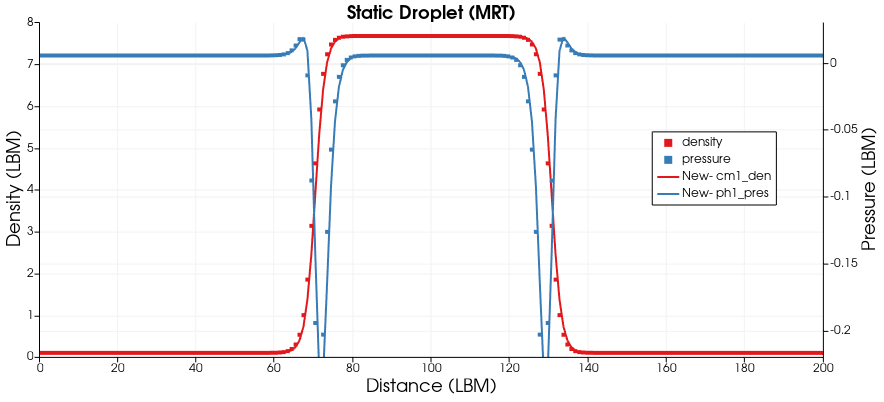
\includegraphics[scale=0.4]{pics/MRT_StaticDroplet_PRho.png}
		\caption{Comparison of pressure and density.}
		\label{fig:val1CMRT}
	\end{figure*}
	 
	\subsection*{What will be done next week?}
	I will finish the MRT validation against Cheng's codes, but this paradigm is becoming more complex every time, as the codes are extensive and each one changes its input parameters. I feel that attach to simpler but extensively reported cases would be better for our purpose. As the MRT code is already running and giving good results (qualitatively), I consider the two-component case is ready to be addressed. The code is already generalized, so the only missing part is to configure the cases and start running and debugging. 
	
	\subsection*{Difficulties}
	\begin{itemize}
		\item The MRT case does not show several oscillations as the BGK does. 

		\item The BGK has only one parameter that relates to the viscosity of the fluid, so I can control how fast the momentum diffuses through this parameter. However, MRT has more parameters, and sometimes they look like \textit{magic-parameters}, that I am still understanding to produce stable simulations.
		\item There are many validation codes, and handling that amount of versions is becoming overwhelming. How can I generate enough trust in the model?
		\item Side note: The phase behavior model I have in C++ started as a class project the last semester for the Advance Programming course, and is the mandatory project for the Thermodynamics course I am taking this semester. That is the reason I am developing the code, and the fact it is in C++ is because I want to improve my proficiency with high-performance programming languages. 
	\end{itemize}


	\pagebreak
	\section*{Feb 14 - Feb 19}
	\subsection*{What was done last week}
	According to the plan from past week, and given the instructions by Dr. Ayala, I ran again the oscillation droplet for BGK and MRT, and compared against my code. After a tough debugging process, I discovered the cause (difference in numerical parameters) of the discrepancies in the MRT case. Now, both codes are providing the same results for the two collision operators (figure \ref{fig:osci}). This debugging process lead me to repeat the Cheng's previous MRT implementation, that although is manual and cumbersome, accelerates considerable the code as no matrix-vector operations are needed. As a parallel example, I ran the case of a falling droplet, that marked the importance to generalize the viscosity as a value per phase.
	
	I skimmed through some papers studying the Marangoni flow with LBM solvers. Part of this search was presented in the Friday's meeting, where I could understand better (not completely) the phase-field model based on the free-energy functional. Although no research related, I consider important to inform that I sent the documentation to apply for a Minor in Computational Science, although last semester I took most of the credits needed for this goal, and only 6 credits are missing for this purpose, apart from the missing research credits I have pending. 
	
	\begin{figure}[h]
		\centering
		\begin{subfigure}{.5\textwidth}
			\centering
			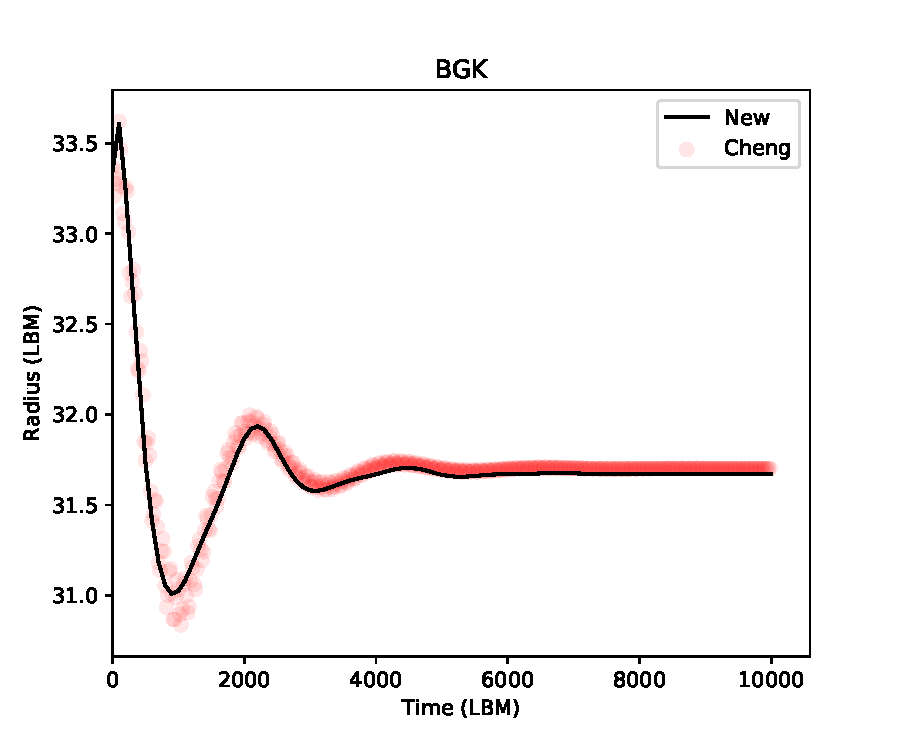
\includegraphics[width=.6\linewidth]{pics/BGKOsc.pdf}
			\caption{BGK}
			\label{fig:sub1}
		\end{subfigure}%
		\begin{subfigure}{.5\textwidth}
			\centering
			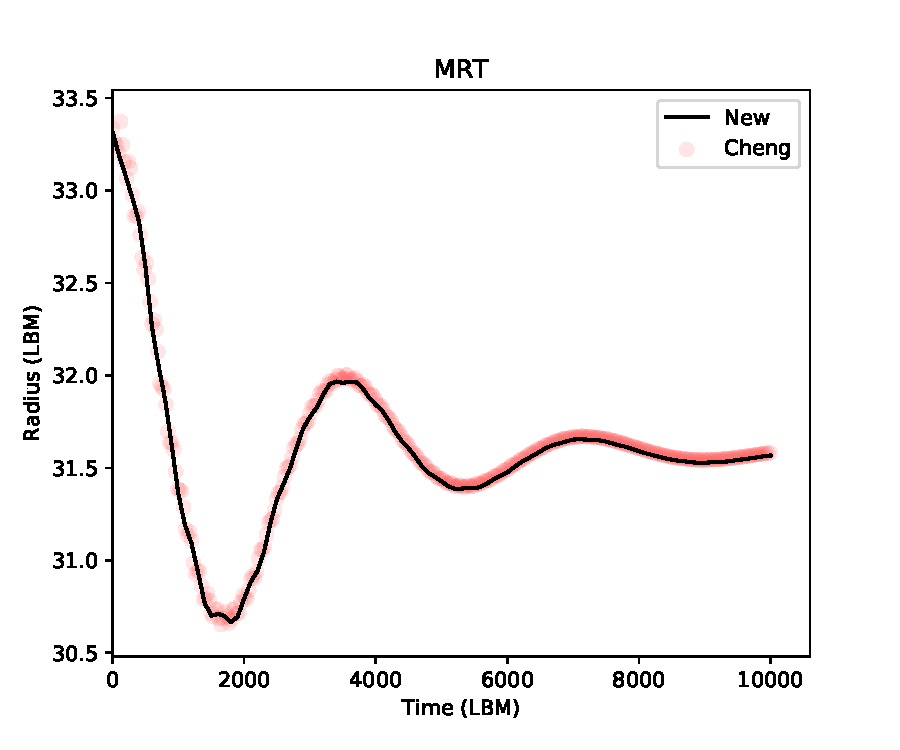
\includegraphics[width=.6\linewidth]{pics/MRTOsc.pdf}
			\caption{MRT}
			\label{fig:sub2}
		\end{subfigure}
		\caption{Oscillation droplet case. Viscosities are different in each case.}
		\label{fig:osci}
	\end{figure}
	
	\subsection*{Difficulties}
	\begin{itemize}
		\item One difficulty raised from the high terminal velocity that a falling droplet reaches due to gravity. I haven't had the time to test a rising bubble (may present a smaller velocity) but it would be a good match example once I fixed the viscosity per phase. In fact, I feel I have not understood the advantages that LBM can provide in terms of physics modeling, and I should be better aware of both its limitations and benefits, compared with the others well-known methods. 
		
		\item I also have had a debugging difficulty with GDB and Fortran, as sometimes the run simply collapse when I intend to access some object's information.
		
		\item I found myself confused with the management of information regarding my own advances and thoughts, and with migrating them from where I was accustom to (Discord, Obsidian).
	\end{itemize}
	 
	
	\subsection*{What will be done next week?}
	I forecast a busy week due to an exam I have on Thursday, the talk given by Dr. Pyrak, two homework for the next week, and a meeting with Dr. Ayala's research group, that includes Cheng as a guest to discuss the LBM difficulties. With the available time, I will start the 2-component case (oscillating droplet). I would like to receive some feedback during next weeks, about the direction we are going with the code and research objectives, maybe in a separate short-meeting between you Dr. Mehmani, and Dr. Ayala. During this week, the meeting with Cheng is particularly important, as there is where I can solve some concerns about LBM that are not clear enough in some books or papers, and where I can connect better with his ideas, and accelerate the paper writing. 
	
	\pagebreak
	\section*{Feb 21 - Feb 26}
	\subsection*{What was done last week}
	This week was predominantly centered around research meetings, talks, and exams. I had a meeting with Dr. Ayala's research group, to show the advances on the new code. One of the conclusions during the meeting was that the outflow boundary condition is still a not-solved problem, as it is no clear what is the implication at the macroscale, the fact of imposing a zero gradient at the mesoscale in only certain directions. The increasing in mass is caused by the bounce back scheme, were the distributions are reflected, causing a net $\Delta m$ non equal zero. In the meeting, they encourage to find the source of mass increasing (if occurring close to the inlet or outlet). Also, recommended to extend the column of fluid for the falling droplet, as the flow generated by the droplet may influence the hydrodynamics of itself using the periodic condition. Cheng also want me to repeat the rotating droplet with my code to see if it can converge. If you remember, Dr. Mehmani, long time ago I showed you a rotating droplet that was gaining momentum and not converging to equilibrium, and Cheng said he had troubles making that case to converge, and is the one I am referring to. It is still needed more exploratory work about the combination of boundary conditions. 
	
	\subsection*{Difficulties}
	\begin{itemize}
		\item I used to employ general correlations for viscosity, such as the Lorentz-Bray-Clark model, that takes into account composition for the viscosity of a mixture. I used this for compositional modeling, but I do not have clear what the implications are in the N-S equations, to apply linear mixing rules. Is the common practice in pore-scale, to treat the viscosity as a linear combination based on densities of the components? I was struggling in deciding which scheme to use, as this may impact: a) The resulting N-S equation that is being reproduced, b) The computational overhead in the code. 
		
		\item No other particular problems were found this week more than the usual about time management.
	\end{itemize}
	
	
	\subsection*{What will be done next week?}
	I will present two exams this week, and I have to finish a report about the phase behavior model in C++. I plan to focus mostly in these three aspects and include the correction to compute the viscosity based on current composition, as this is important to correct the previous multiphase simulation cases, and to address the 2-components simulation.

	
	\pagebreak
	\section*{Feb 28 - Mar 13}
	\subsection*{What was done last week}
	During these two weeks, the front where I spent most of the time was the programming of functionalities needed for addressing the two-component multiphase simulations. I programmed the viscosity interpolation based on density, using two given reference viscosities. I tried to use this modification to make the falling droplet case to converge. I was planning to modify the viscosity of the surrounding vapor high enough to equal the gravity force with the drag force, but I have not found the combination of parameters that produces a stabilization with a terminal velocity within the range  valid for LBM. I skipped this difficulty and left this front in stand-by, in order to prioritize the oscillating droplet using two components. For this purpose, I (a) incorporated the initialization based on composition fields, (b) reported the fluxes at boundary nodes to check the mass conservation (strictly speaking, this still is not a material balance criterion), (c) improved the routines computing the topology of the mesh, to use this information for the Shan-Chen force computation (it depends on neighbors' pseudopotential), and (d) run static and oscillation droplets to start the validation process. With these changes, the force is in agreement with the boundary conditions imposed for the flow, and the implementation for immiscible flow, and fluid-solid interactions are in a 50\% of development.
	
	\subsection*{Difficulties}
	I found out that the outflow boundary conditions I implemented have a mistake in their mathematical form. As the boundary conditions and their generality were not the main focus during the code construction, I only tested rigorously the ones more used by the validation cases (pressure, velocity, and periodic). Now, I know where to find the correct mathematical description of such conditions in order to apply them for the multi-component case. However, for the oscillating droplet I can still work with the periodic boundary conditions. A second difficulty was related with computing the net flux across the boundaries, which I computed as:
	\begin{equation*}
		\dot{m}_b = \sum_{l(b)} \rho_l (\mathbf{u}_l \cdot \mathbf{n}_l) A_l 
	\end{equation*}
	where $l$ stands for a block in the boundary $b$. As the solution for $\rho$ and $\mathbf{u}$ are given at the center of the lattice, this flux is not representative of the real boundary, and a correction for the dynamic variables must be performed. 
	
	\subsection*{What will be done next week?}
	I plan to compare the results of the oscillating droplet with the Cheng's code and his previous paper, and against the analytical solution for the period of oscillation, at the same time I analyze the assumptions behind this equation, and put down the findings during the validation.
	
	\pagebreak
	\section*{Mar 14 - Mar 20}
	\subsection*{What was done last week}
	The main objective of the week was the validation of the oscillation period. For this purpose, I previously had the main simulation, but still the simulations of static droplets with different radii were missing (to compute the interfacial tension, IFT), and no analysis of the oscillation period was done in the last week. These were the two fronts covered with the following results. The Figure \ref{fig:laplace} shows the validation of the Young-Laplace equation, obtaining a surface tension of 0.12141 in LBM units, and is also shown the LBM simulation of the oscillating droplet, compared with the Cheng's code. There is an offset of 3.6 units in the radius, that is product of the increasing mean diameter, an effect that is not seen in Cheng's results. This effect can be better seen in the Figure \ref{fig:2cOsc}, where the mean radius is computed as $R_e = \sqrt{R_x R_y}$. To obtain the frequency, a Fourier transform was employed, where a peak at 10010 T was obtained. 
		\begin{figure}[h]
		\centering
		\begin{subfigure}{.5\textwidth}
			\centering
			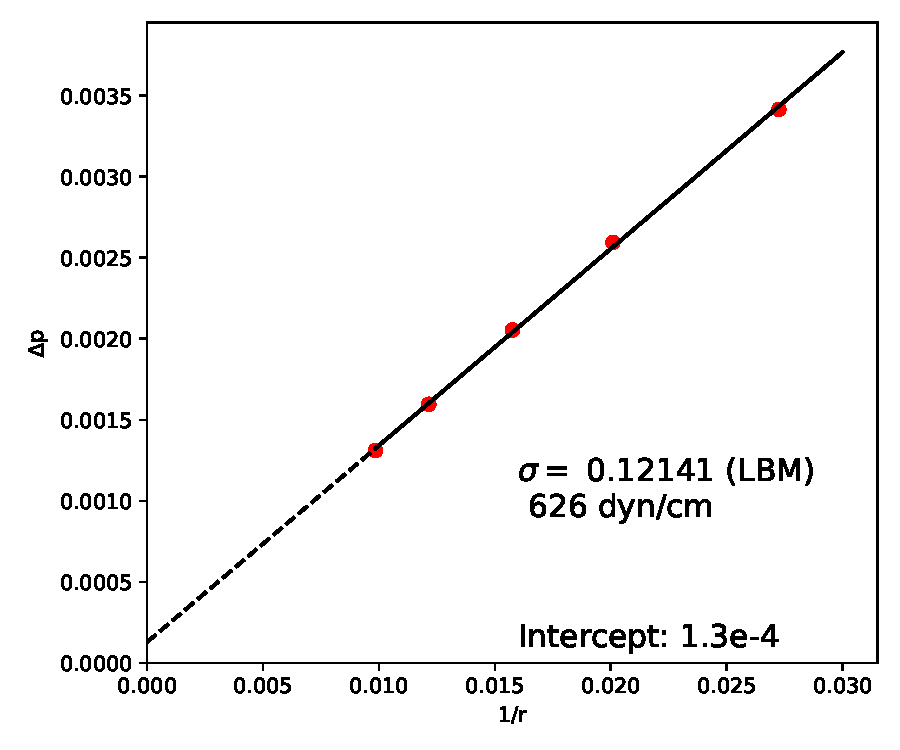
\includegraphics[width=1\linewidth]{pics/IFT.pdf}
			\caption{Young-Laplace validation}
		\end{subfigure}%
		\begin{subfigure}{.5\textwidth}
			\centering
			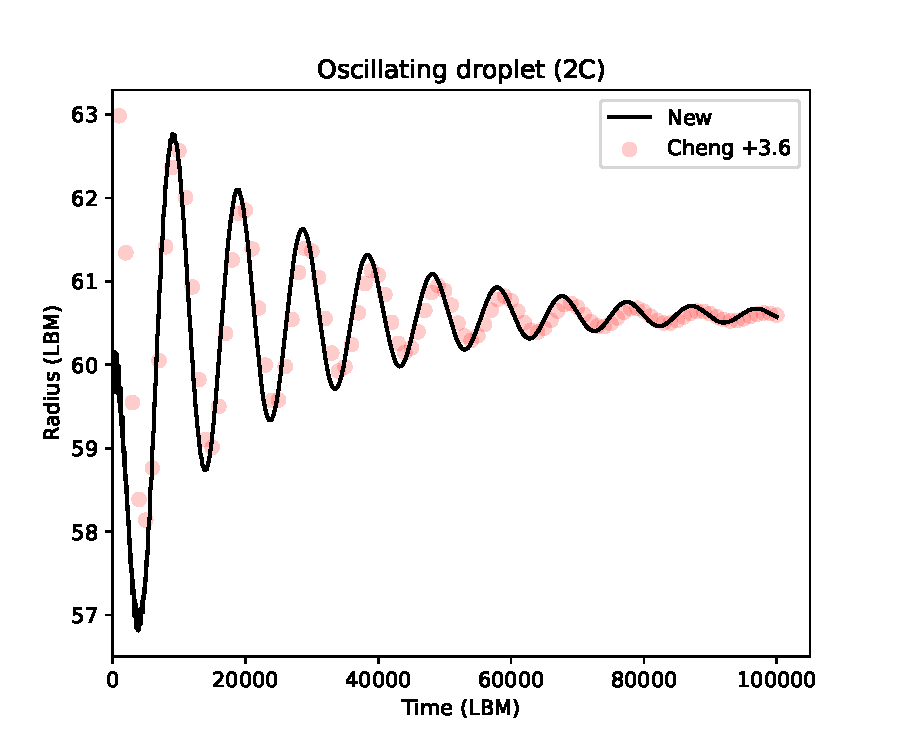
\includegraphics[width=1\linewidth]{pics/2cOsc.pdf}
			\caption{Comparison with Cheng.}
		\end{subfigure}
		\caption{Young-Laplace and Comparison with Cheng.}
		\label{fig:laplace}
	\end{figure}
	
	\begin{figure*}[h]
		\centering
		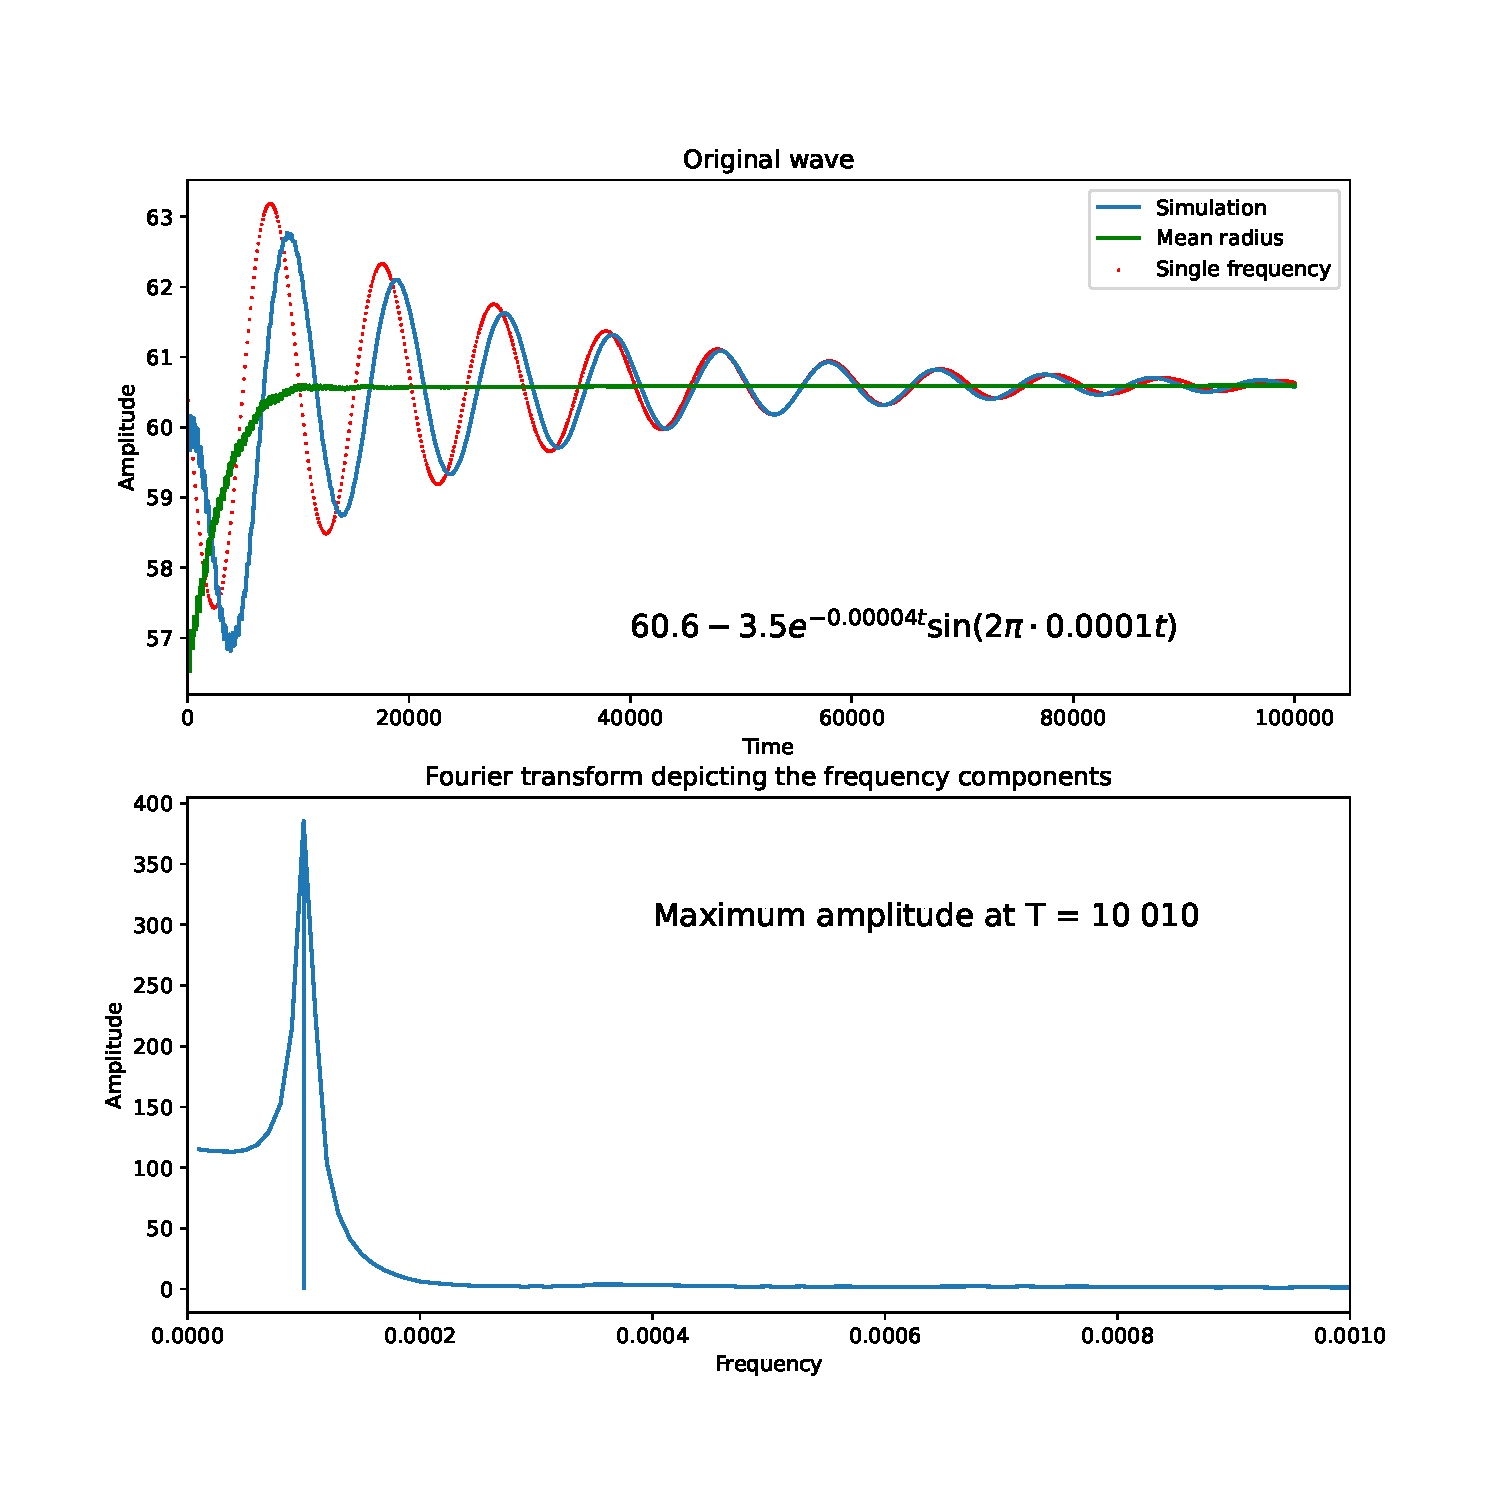
\includegraphics[scale=0.5]{pics/fourier.pdf}
		\caption{Oscillations and evolution of the mean radius. Fourier transform.}
		\label{fig:2cOsc}
	\end{figure*}
	
	As a summary, the equilibrium radius is equal to 60.59, the interfacial tension to 0.12141, the liquid density to 8.277, and the numerical period equal to 10010 T. Now, to compare against the analytical period, we have the equation:
	\begin{equation}
		T_a = 2 \pi \left[ \frac{n (n^2-1) \sigma}{\rho_l R_e^3} \right]^{-0.5}
	\end{equation}
	That gives a period of 9989 T, that produces an error of 0.2\%. I found a problem with Cheng's paper, where the exponent of -0.5 is missing. 
	
	\subsection*{Difficulties}
	I may have one problem during the initialization stage. All the simulations are depicting an increase in the droplet radius, so the first oscillations are not centered around the equilibrium value, as if the interface were to accumulate energy at time zero. I am trying to figure out if this is product of the interface size, the method used to locate the interface, or an initialization problem. This effect was not present during the single component case.
	
	\subsection*{What will be done next week?}
	I will work on the problem of the increasing radius to discover what is causing this effect, which I consider critical to keep advancing to other cases. I also need to test the same simulation, activating a correction term of MRT that reduces spurious currents, and that is present in some of the Cheng's simulations.
	
	\pagebreak
	\section*{Mar 21 - Mar 27}
	\subsection*{What was done last week}
		The purpose of this week was to present the advances in the validation cases to the Dr. Ayala research group and decide how to continue in the direction of finishing the cases that will go to the paper. To be honest, I realized that I have been working in a dispersed way, where part of my work, focused on simulation, was spent in finding the cause of not matching as I would like, the Cheng's results. Although the analytical solutions have matched really well, I keep thinking that to drop all the legacy codes, I should be able to match the cases that were left by Cheng, or at least explain the differences. Simultaneously, I ran some initial cases for the rising bubble to validate the model under the action of gravity. Before going further in this direction, I need to do a bibliographic review that will be better stated in the last section of the report. 
		
	\subsection*{Difficulties}
	
	Although I could relax the demand to myself of matching perfectly the Cheng's code, I am still struggling with the droplet increase during the first cycle of oscillations in the multi-component case. I did not experience this effect during single-component simulations, but comparing a very refined simulations (in terms of time resolution), turns out that the increase appears after 1000 time iterations, and only in one of the droplet sides (right). After a while, the left side also increases, and then both are stable. It is worth saying that this difference is about half the size of the diffuse interface, but, although it sounds small, by where the differences are in the codes and the phenomenological nature of this effect\footnote{I am assuming this is not product of numerical errors}, there should be not discrepancy. Regarding the raising droplet, I realized that an uniform force is only valid to model gravity when there are not periodic conditions in the force direction.
	
	\subsection*{What will be done next week?}
	I consider important to pause and make some decisions before taking the next step with more confidence and to avoid the dispersivity feeling. First, I will do a bibliographic review of the oscillating droplet to see how other authors have presented this kind of simulations with LBM or other modeling techniques. Also, I will gather several approaches to include the gravity in the multi-phase approach, where I have found a couple of methods. In summary, this week should be focused on: bibliographic review of droplet oscillations and rising bubbles with multiphase models. Regarding to code, I need help with deciding if it is important to keep looking for the cause of the increasing radius (again, it happens during the first complete oscillation, but I have not read this in other papers). If it is relevant, I need to propose a systematic way to find the reason, because up to now, I have tried many things that have not solved the "problem" and now any other try will increase the entropy of this search.
	
	\pagebreak
	\section*{Mar 28 - Apr 11}
	\subsection*{What was done last week}
	I searched for papers addressing the same type of simulations I have in mind, to get a better idea of how to report my results and what are the main flow characteristics that are analyzed and presented, and compare the LBM approaches with other methods that are used for the same simulation setup. I did this for the oscillating droplet and the rising bubble. 
	
	I designed some cases for the raising bubble, based on the flow regimes of interests in this problem. There is experimental data showing different bubble shapes, depending on the Reynolds ($R_e = u d_b/\nu$) and Bond ($B_o = g \Delta \rho d^2_b / \sigma$) numbers. Three main shapes are depicted as a function of these numbers: spherical, elliptical, and dimple-shaped. I was able to reproduce the spherical and elliptical regimes (the later eventually moves away from the center axis, showing that there is a non symmetric effect in the code that, although honors the relevant physics, causes an offset in the center of gravity of the system). The dimples were not possible to run, as the gravity force had to be increased to a number that, being simultaneously applied with the Shan-Chen force, creates an instability and the simulation diverges. I tried to increase the bubble size to increase the Bond number, but this implies larger simulation domains and longer runs. A best approach to increase the Bond number will be to play with the thermodynamic setup, to decrease the surface tension predicted by LBM. Dr. Ayala encouraged me to print the asymmetry in the domain of a relevant variable (density, velocity, a distribution function) to find the source of the symmetry breaking, where I did not discard to be product of the high velocity regimes, where the velocities approach to high Mach numbers, and the difference in precision becomes relevant for stability.
	
	\begin{figure*}[h]
		\centering
		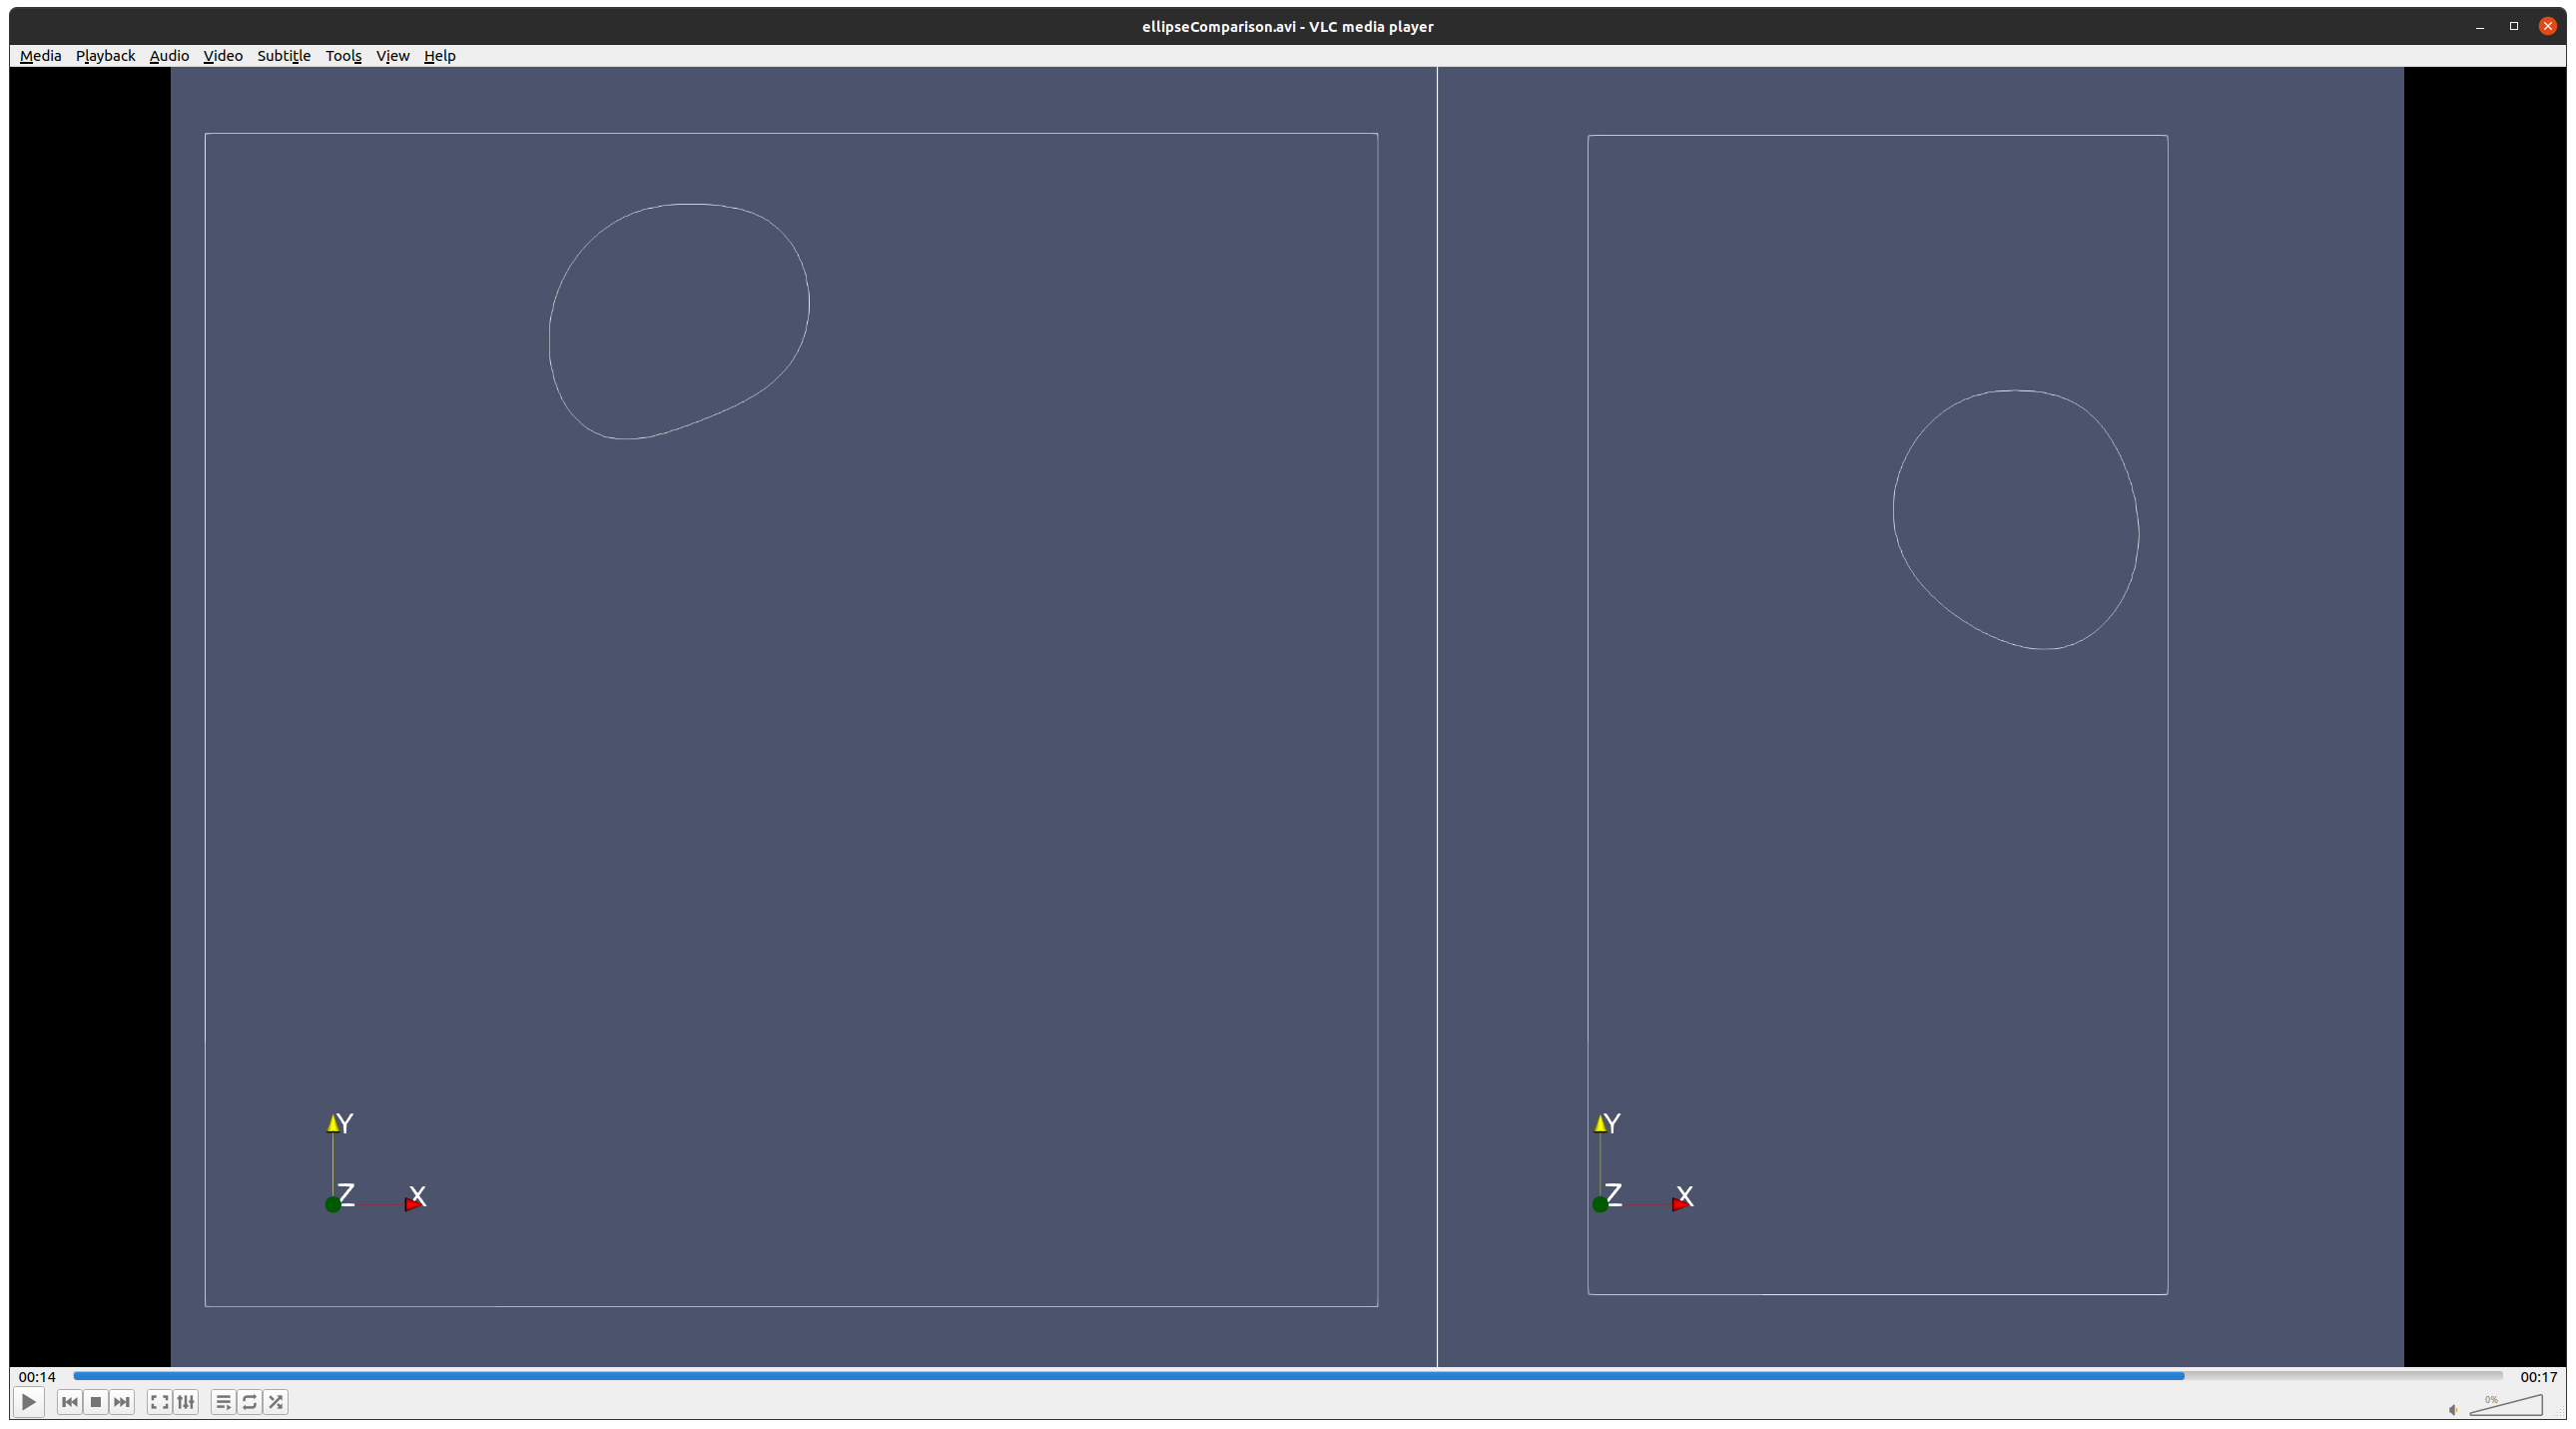
\includegraphics[scale=0.1]{pics/ellipseCompMove.png}
		\caption{Elliptical regimes after symmetry is broken.}
		\label{fig:ellipseCompMove}
	\end{figure*}
	
	Finally, as part of a homework for the PNG 518 course, I solved the advection-dominated equation of a solute reacting with the rock, using both Laplace and the Method of Characteristics. I consider this relevant for the Qualifying exam, where I expect questions of this type, and this was one of my concerns weeks ago in the PNG 501 course. 
	 
	\subsection*{Difficulties}
	The difficulties are related with the dimple-shaped regime, where further reading will help to determine how others have modeled the problem using LBM. At a first glance, it looks like others have used the immiscible no-thermodynamic consistent approaches to model the two-phase behavior, what may help to improve stability for higher magnitudes of secondary forces (the thermodynamic consistency may be more sensible to small perturbations). 
	
	
	\subsection*{What will be done next week?}
	
	I signed up to be a judge in a Undergraduate Poster Competition this April 11th, to start familiarizing with other's research and judgment environment. Regarding research, I will evaluate the symmetry breaking that is taking place, and will keep going with paper reading. I will be preparing a presentation in SPH, which was the topic I was assigned in the course EME 521. This is not part of my research, but is a mandatory project, and I consider it relevant to understand how other Lagrangian methods work and find relations with LBM at some point if necessary.
	
	
	\pagebreak
	\section*{Apr 11 - Apr 17}
	\subsection*{What was done last week}
	The three fronts of this week were the work on SPH, the identification of the asymmetry source in LBM, and coding on the phase behavior model.\\
	Regarding the SPH topic, I finished writing a quick presentation about the concepts behind SPH, the concept of the discrete interpolation and the interpolation-based gradients, which open the door for a Lagrangian description of the Navier-Stokes equations. Also, I read about the implementation of boundary conditions in this type of systems. I find the concept of interactive particles in SPH, very similar to the concept of interacting probability distribution functions in LBM, being SPH less exposed to the coupling to cubic EoS for fully-thermodynamic consistent models.\\
	Evaluating symmetric simulations, I found the reason for asymmetry in my LBM code. The source was a silly geometrical misinterpretation of my initialization routines, which were taking the centroid of the lattice as if it were the left-lower corner. Although this does not explain the increasing radius in the oscillating droplet simulations, the correct implementation solved the asymmetry and prevented the bubble from deviating from the central axis. However, some aspects were recognized here: a) the magnitude of asymmetry now is of the order of machine precision (1e-14), b) the asymmetry can propagate to values up to 1e-13, but if instability regions are approached, the asymmetry can develop to magnitudes comparable to the variable being analyzed (densities, velocities) and then the simulation diverges. Fixing the asymmetry, I could evince that the walls were affecting the flow regime of the rising bubble, so I am reading other studies to find the aspect ratio that most of other researchers have used in their approaches. As the simulation runs are taking longer as we approach to more complex cases, I programmed a progress bar with an estimation of the time it will take to finish the run, which will be useful when submitting jobs to the PSU-computing center, to control the time and decide when to save a restart and keep the simulation going with a new execution.\\
	I finished the last module of my phase behavior model, and I will be cleaning the code and the repository to have a neat library that can be further coupled to our research and LBM code if necessary.\\
	I took the suggestions from Dr. Mehmani about what makes a good summary when reading papers and I think I have now my own methodology that suits my preferences in terms of the hardware and software I use for annotating documents. I will embed the proposed sections on an extra page in the software I use for annotating papers, and I will export that page (or extra pages if needed) to a single document containing all the documents I have read about a particular area. I like this method as I usually read from my tablet in different locations and I can keep the notes attached to the original document, which Dr. Ayala requires to have in our own Teams space.
	
	\subsection*{Difficulties}
	No particular difficulties arose this week, more than evidencing the cost of changing tasks during the day (or even the week). I am certainly trying to keep my schedule restricted to very specific tasks, while planning my activities as a series of specific goals. 
	
	\subsection*{What will be done next week?}
	I will be preparing some exams and works for my classes, but in terms of research, I will be condensing all the information I have gathered (reading, fixed problems, preliminary simulations) in a single presentation, to present it to Dr. Ayala in order to take action and identify what has to be done before meeting with Cheng again, and to show the capabilities of the multiphase model to the Dr. Mehmani research group next week. 
	
	\pagebreak
	\section*{Apr 18 - Apr 24}
	\subsection*{What was done last week}
	I summarized the simulation procedure that I was developing during previous weeks, and presented these results to the Dr. Ayala's research group. The case can be presented as:
	
	\textbf{Goal}: Test the pseudopotential approach for partially misc. mixtures, under the action of gravity.
	\textbf{Methodology}: Test different flow regimes based on Bond (Eotvos) and Morton numbers. Validate the \textbf{terminal velocities and bubble shapes} against experimental and simulation data.
	\begin{equation*}
		R_e = \frac{\rho_l u_b d_b}{\mu_l}
	\end{equation*}
	\begin{equation*}
		B_o = \frac{g \Delta \rho d_b^2}{\sigma} \,\,\,\, 	M_o = \frac{g \Delta \rho \mu_l^4}{\sigma^3 
			\rho_l^2}
	\end{equation*}
	
	
	A thermodynamic state fixes $\rho, \Delta \rho, \sigma$. At a given temperature, in a single component case, some values are provided ($\rho, \Delta \rho$) and others can be obtained by simulating the static droplet ($\sigma$). 
	
	\textbf{Procedure}: a) Select $B_o$. b) Calculate the gravity as $g = \frac{B_o \sigma}{\Delta \rho d_b^2}$. c) Select $M_o$. d) Calculate $\mu_l^4 = \frac{M_o \sigma^3 \rho_l^2}{g \Delta \rho }$. e) Select the viscosity ratio f) Calculate $\mu_g = \mu_l * \frac{\mu_g}{\mu_l}$.
	
	I followed the procedure for the single-component and multicomponent case, finding the following:
	\begin{itemize}
		\item The spherical regime was observed at the $B_o$ number predicted by the experimental studies.
		\item The ellipsoidal shape gets distorted by the presence of the wall. As the $R_e$ is small, this approaches Stokes flow, where the flow extend to the whole domain and the non slip condition affects the streamlines. However, some studies were able to reproduce the ellipsoidal regime. 
		\item The current LBM implementation makes prohibitive reaching high $B_o$ numbers, where the spherical cap is formed. That regime may be achieved by increasing the bubble radius (higher computational domain).
		\item The multicomponent approach with Shan-Chen has less flexibility to play with surface tension, reducing the degrees of freedom, and being prone to instabilities.
		\item Single component and multicomponent cases have similar features. The multicomponent case tends to be more unstable, but depicts better bubble behaviors, such as bubble splitting.
	\end{itemize}
	
	\begin{figure*}[h]
		\centering
		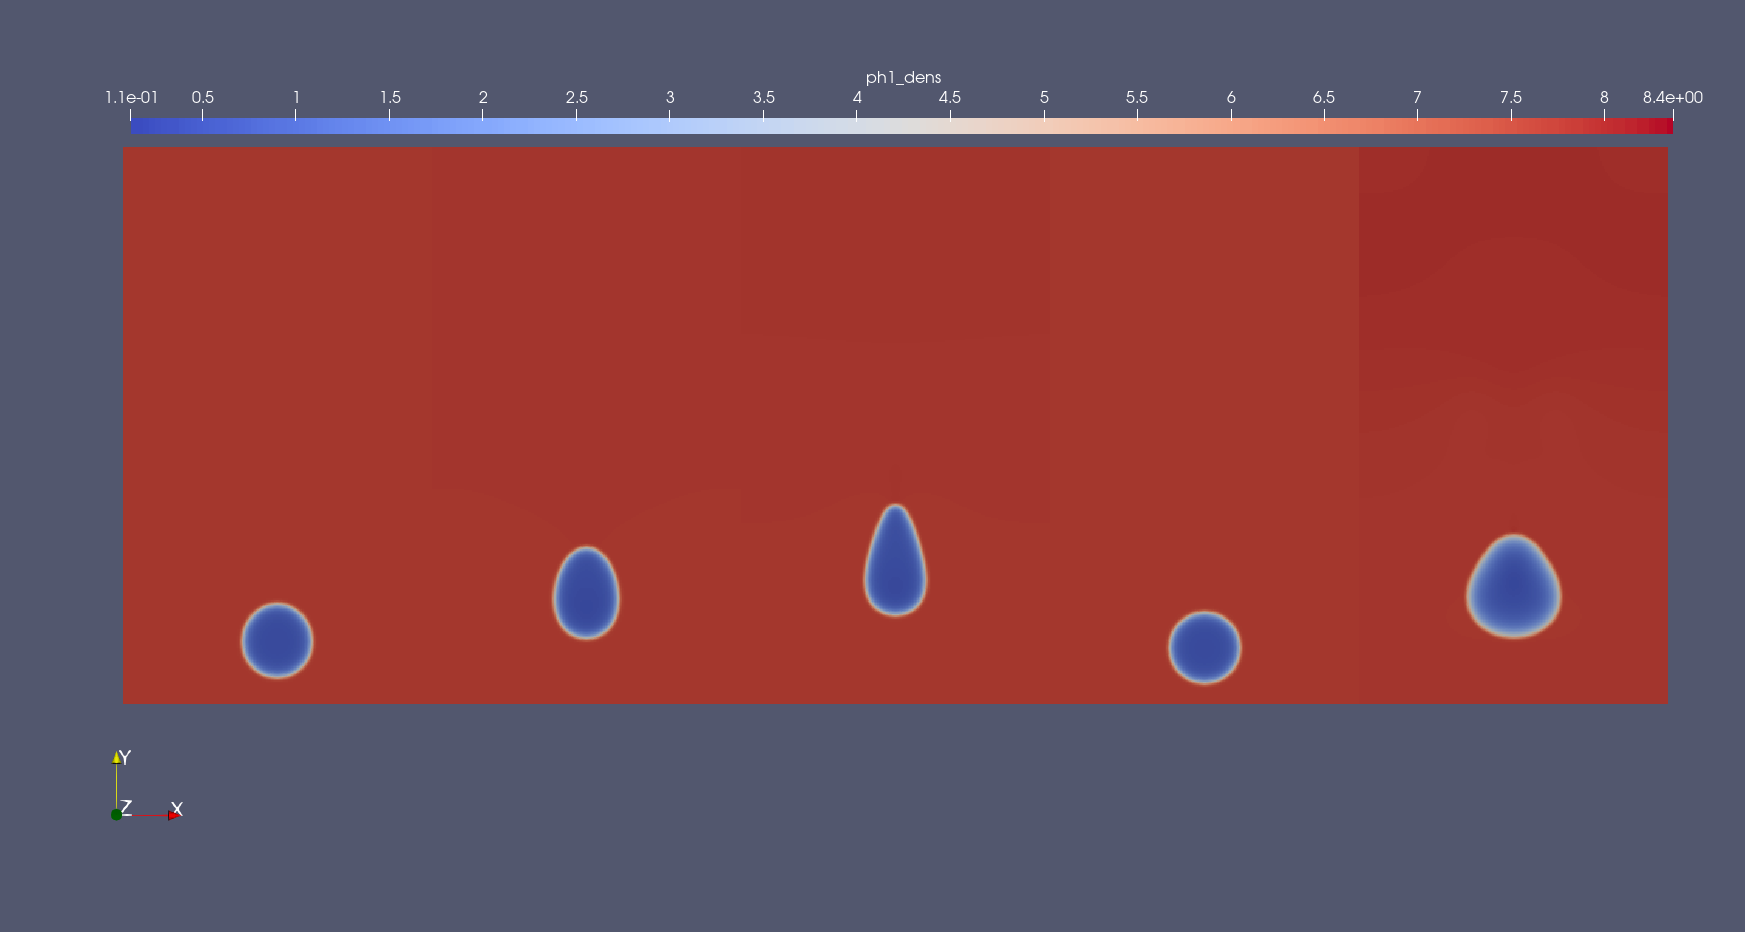
\includegraphics[scale=0.2]{pics/risingCompDen.png}
		\caption{Bubble shapes.}
	\end{figure*}

	\subsection*{Difficulties}
	One difficulty was related with designing the simulation cases to avoid creating more than those needed. As we can change many parameters to arrive to the same flow regime, sometimes I found myself loosing track of the cases I ran, or loosing the connection with the previous ones. However, I think the best solution is simply to always write down what will be done, and attach to the plan as much as possible.\\
	
	A second difficulty was the crashing of my personal computer. I had bought a simple machine for home-working which currently has Windows in it\footnote{I know, a Mac would have been better, but this was a gaming machine for half of the price!}, and realize that the way I compile my code is not cross-platform. I feel that it is important to learn how to write CMake Files, and use this tool to be able to compile in different OS. I actually enjoy working in Linux, and I find much easier to compile my codes with external libraries in this OS. I have to decide if keep working cross-platform or switching again to Linux, what is not a minor decision as in the future others may be writing code in the current LBM implementation. 
	
	\subsection*{What will be done next week?}
	Including this and next weeks, the following are part of the actions suggested to overcome the current difficulties. First, switch to periodic boundary conditions, using a few (or one) solid block somewhere, or check if the current implementation of gravity ($f_g = g (\rho - \rho_l)$) solved the acceleration of the whole system. The purpose is to see if the ellipsoids can be seen better with peroidic BCs. Second, it is desirable to go back to the original Shan-Chen, which was used in some papers to model the rising bubble. Here, we will check if those results are reproducible and conclude if the ellipsoid problem is product of the proposed Shan-Chen force-splitting scheme. Third, there is a correction to the LBM formulation to eliminate the ideal pressure from the recovered Navier-Stokes equation, what may simplify the expression for the current Shan-Chen force and thus avoid instability problems. I will finish the presentation on Friday for the Dr. Mehmani research group, and conclude some activities before entering to the finals week.
	
	\pagebreak
	\section*{Apr 19 - May 8}
	\subsection*{What was done last week}
	The last two weeks were used primarily to finish the semester's deliverables and present final exams. From the course in Mathematical Modeling (EME-521), I could grasp some ideas for multiphase models. In particular some relevant references about the Cahn-Hilliard equation, which looks to be the future implementation to the LBM model to better address the problem of thermodynamic inconsistency. I read a highly cited paper in LBM, He X., Doolen G.D., Thermodynamic Foundations of KInetic Theory and Lattice Boltzmann Models for Multiphase Flows. 2001. Journal of Statistical Physics. They propose that the source of inconsistency in the Shan-Chen force is due to considering only the nearest neighbors in the interparticle potential approach. Also, they were aware of the problem of fixed interfacial tension once the force parameter $G$ is fixed. Let's remember that this reduces flexibility to simulate a wider range of flow regimes. From this paper I derived some questions about thermodynamic systems with curved surfaces. Finally, I was preparing the second part of my presentation to the research group, where I could receive some feedback about the content and the way I present. Summarizing the recommendations and my own conclusions from the presentation and past reading:
	
	\begin{itemize}[leftmargin=*]
		\item The derivation of the equilibrium distribution function based on Hermite polynomials, the theory of multiscale expansion to obtain the Navier-Stokes equation from LBM, and the theory of liquids and vapor from a molecular perspective (capillarity), are some of the theoretical fields I may want to cover in the near future to have better tools to propose an improved model in LBM. This includes the theory of Cahn-Hilliard and its solution with the Phase-Field method. 
		
		\item Keep only one ellipsoidal regime and try different force implementations (and viscosity rations) to see if the bubble tip (prolonged one) does not appear and the correct shape is observed. 
	\end{itemize}
	\subsection*{Difficulties}
	The difficulty observed this week was no other than the one from previous weeks: the tendency to diverge once I finish some heavy workload such as the courses or final exams. However, as before, the solution seems to be to attach to the plan I had before: keep reading my selected literature about dynamic multiphase modeling with LBM, and keep the plan for the model, as will be mentioned in the next section.
	\subsection*{What will be done next week?}
	These weeks I was away from the code, as I was focused on other activities. However, I will go over the code again, to implement the immiscible Shan-Chen force (not consistent, but some papers have modeled successfully the rising bubble with it), and the reproduce some published results before going deeper with the multicomponent Shan-Chen force. 
	
	\pagebreak
	\section*{May 9 - May 15}
	\subsection*{What was done last week}
	During this week, several code implementations took place, while attempting to obtain a stable simulation of the rising droplet. In this sense, the Shan-Chen force was implemented in its more generic way, accounting for the interaction between all components:
	\begin{equation*}
		\mathbf{F}^i (\mathbf{x}) = - \psi_i \sum_j \sum_l G_{i,j} \psi_j (\mathbf{x} + \mathbf{e}_l \Delta t) w_l \mathbf{e}_l \Delta t
	\end{equation*}
	This force was validated for a single droplet, employing several pseudo-potentials $\psi$ recommended in literature, and is giving the reported results for the equilibrium densities in the two bulk phases. The reference paper for bubbly flow, proposes a force that keeps the total acceleration of the system equal to zero in periodic domains, $\mathbf{a}_g =  \mathbf{g} (1- \bar{\rho}/\rho)$, where $\bar{\rho}$ is the average density of the system. First simulation attempts show the rising of the bubble using these two forces, but further work on the simulation setup is required. Other improvements were done to reduce some arithmetic operations in the code, generalize the input parameters, and to produce folder-separated outputs, what facilitates the data transferring between computers. Also, the time-stepping was programmed to be set to values different than 1. However, when reduced, the single droplet diffuses and converges to an uniform density map. This may be product of a reduction in the magnitude of the force applied, avoiding the spinodal decomposition of the components. 
	
	\subsection*{Difficulties}
	The gravity force used here, accelerates slightly the liquid phase, proportional to the difference between its density and the average density. So, it is required to initialize the domain with a small gas bubble, to reduce the acceleration of the liquid phase, and improve stability. Finally, I found a convergence of topics that look like the foundations to understand the physics behind the interface behavior. These are the thermodynamic of interfaces (which Dr. Ayala already committed to have a discussion about), calculus of variations, and functional analysis. To be honest, two of the latter are still blurred to me, so I would like to spend part of the summer studying these topics, and so be able to write a well grounded proposal for my qualifying.
	
	\subsection*{What will be done next week?}
	I plan to reproduce the same scenarios than those presented in the reference used for the Shan Chen force, and those presented using the multi-component scheme that was developed by Cheng, which were presented in previous weeks. I will try to convert my implementation to be implicit, although I am not sure about what to do with the streaming step, which is one of the more computationally costly. Besides, I will make a plan for studying for the qualifying exam. I will check the topics to select the relevant ones for me, and start designing a reading routine. 
	
	%\pagebreak
	%\section*{ - }
	%\subsection*{What was done last week}
	%\subsection*{Difficulties}
	%\subsection*{What will be done next week?}
	\printbibliography % Be sure to remove access date and months from the .bib file
\end{document}